\documentclass{home_assignment}
\usepackage[acronym,nogroupskip]{glossaries}
\usepackage[hidelinks]{hyperref}
\makeglossaries
\newacronym{it}{IT}{Information Technology}
\newacronym{ict}{ICT}{Information and Communication Technology}
\newacronym{gdp}{GDP}{Gross Domestic Product}
\newacronym{aws}{AWS}{Amazon Web Services}
\newacronym{gcp}{GCP}{Google Cloud Platform}
\newacronym{gea}{GEA}{Government Enterprise Architecture}
\newacronym{un}{UN}{United Nations}
\newacronym{ibm}{IBM}{International Business Machines Corporation}
\newacronym{ngo}{NGO}{Non-Governmental Organization}
\newacronym{www}{WWW}{World Wide Web}
\newacronym{ntc}{NTC}{Nepal Telecom}
\newacronym{egmp}{eGMP}{e-Governance Master Plan}
\newacronym{ftth}{FTTH}{Fiber to the Home}
\newacronym{atm}{ATM}{Automated Teller Machine}
\newacronym{abbs}{ABBS}{Any Branch Banking Service}
\newacronym{isp}{ISPs}{Internet Service Providers}
\newacronym{pan}{PAN}{Permanent Account Number}
\newacronym{g2c}{G2C}{Government to Citizen}
\newacronym{g2b}{G2B}{Government to Business}
\newacronym{g2e}{G2E}{Government to Employees}
\newacronym{g2g}{G2G}{Government to Government}
\newacronym{hlcit}{HLCIT}{High Level Commission of Information and Technology}
\newacronym{dbms}{DBMS}{Database Management System}
\newacronym{nitc}{NITC}{National Information Technology Center}
\newacronym{moest}{MoEST}{Ministry of Education, Science and Technology}
\newacronym{moic}{MoIC}{Ministry of Information and Communications}
\newacronym{moga}{MoGA}{Ministry of General Administration}
\newacronym{mof}{MoF}{Ministry of Finance}
\newacronym{eta}{ETA}{Electronic Transaction Act}   
\newacronym{itu}{ITU}{International Telecommunication Union}  
\newacronym{egdi}{EGDI}{e-Government Development Index}
\newacronym{covid}{COVID-19}{Corona Virus Disease of 2019}

\newcommand{\step}[2]{
    \textbf{Step #1:} \textit{#2}
        \begin{figure}[H]
            \centering
            \includegraphics[width=\linewidth]{../Figures/steps-#1}
            \caption{#2}
            \label{fig:step-#1}
        \end{figure}    
   
}
\begin{document}
    \titlePage{S3 Versioning, AWS Glacier and Static Website Deployment on AWS S3}{August 30, 2021}{Basanta Joshi, Ph.D.\\Dipak Poudel}   
    \pagenumbering{roman}
    \tableofcontents
    \clearpage
    \phantomsection
    \addcontentsline{toc}{section}{\bfseries{List of Figures}}
    \listoffigures
    \clearpage
    \phantomsection
    \addcontentsline{toc}{section}{\bfseries{List of Abbreviations}}
    \printglossary[type=\acronymtype,nonumberlist,title={List of Abbreviations}]
    \clearpage
    \pagenumbering{arabic}
    \section{S3 Versioning}
    Amazon \acrlong{s3} (Amazon \acrshort{s3}) is the object storage service provided by \acrshort{aws}. Objects are stored in a S3 bucket, whose versioning is disabled by default. \acrshort{s3} versioning, or simply versioning is a method that allows users of \acrshort{s3} buckets to keep multiple versions of an object in the same \acrshort{s3} bucket. It is particularly useful for,
    \begin{enumerate}
        \item Avoiding accidental deletion of an object as it creates a delete marker on the latest version of the deleted object essentially making the delete marker object the current version.
        \item Avoiding unintentional overwriting of an object as it creates a new version of the object with the same key rather than overwriting the existing object.
    \end{enumerate}
    A note-worthy point is that, \acrshort{s3} versioning is disabled by default, so if an user wishes to have versioning enabled, they need to do it either during bucket creation or at a later time. 
    \begin{figure}[H]
        \centering
        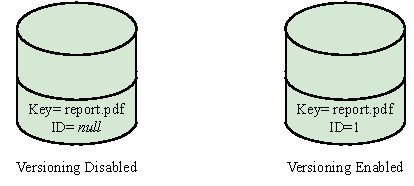
\includegraphics[scale=1.3]{../Figures/versioning_enabled}
        \caption{\acrshort{s3} versioning disabled versus enabled}
        \label{fig:enabled}
    \end{figure}
    Objects placed in buckets with versioning disabled have their ID set to \textit{null}. If a bucket contains objects prior to the enabling of the versioning, the objects will still have their IDs marked as \textit{null}. Any new objects that are PUT in the bucket will get an auto-generated version ID that are composed of various unicode, UTF-8 encoded, URL-ready, opaque strings. To explain \acrshort{s3} versioning, simpler IDs are used in this report.
    This ID distinguishes the different versions of the same key. \\
    \acrshort{s3} buckets can exist in one of the following states,
    \begin{enumerate}
        \item Versioning disabled (default)
        \item Versioning enabled
        \item Versioning suspended
    \end{enumerate}
    Once a bucket's versioning is enabled, it can never be disabled, rather can only be set to a versioning suspended state by an user with the required permissions.
    \subsection{Different scenarios in versioned bucket}
    \subsubsection{PUT an object in versioning enabled bucket}
    When an user PUTs an object in a versioning enabled bucket with the key of an existing object, rather than overwriting the object, the new object is stored with a new version ID and becomes the latest version of that object. This way accidental overwriting is prevented.
    \begin{figure}[H]
        \centering
        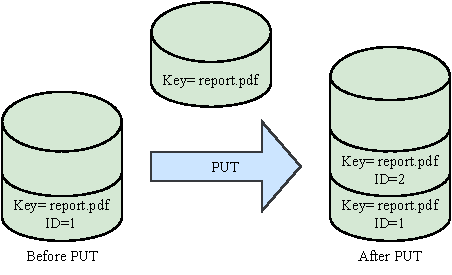
\includegraphics[scale=1.3]{../Figures/versioning_put}
        \caption{PUT an object in versioning enabled bucket}
        \label{fig:put}
    \end{figure}
  

    \subsubsection{DELETE an object from versioning enabled bucket}
    When an user DELETEs an object from a versioning enabled bucket, rather than deleting the object, a delete marker is inserted with a new version ID and becomes the latest version of that object. This way accidental deletion is prevented as the older versions of the object are still stored in the same \acrshort{s3} bucket.
    \begin{figure}[H]
        \centering
        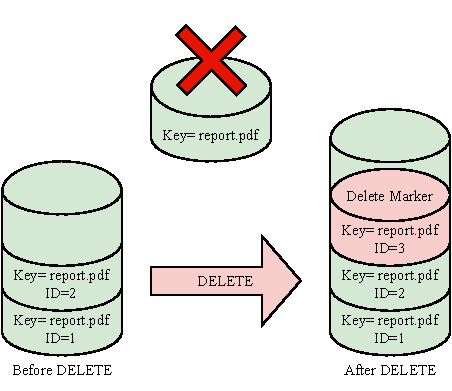
\includegraphics[scale=1.3]{../Figures/versioning_delete}
        \caption{DELETE an object from versioning enabled bucket}
        \label{fig:delete}
    \end{figure}
  
    \subsubsection{GET an object from versioning enabled bucket}
    Since GET request returns the latest version of an object, a simple GET request to retrieve the report.pdf object in the current situation would return a '404 No Object Found' error since the latest version is a delete marker. This is because the delete marker identifies the object as deleted although there are older versions of the object existing in the same bucket. If the user wishes to retrieve an older version of the object that is not marked as deleted, then the GET request must be modified to point to the exact unique version ID that the user wants to get.
    \begin{figure}[H]
        \centering
        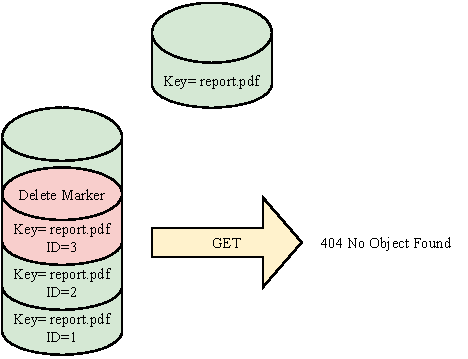
\includegraphics[scale=1.3]{../Figures/versioning_get}
        \caption{GET a delete marked object}
        \label{fig:get}
    \end{figure}

    \begin{figure}[H]
        \centering
        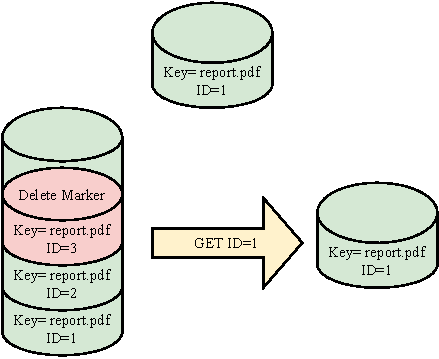
\includegraphics[scale=1.3]{../Figures/versioning_get_id}
        \caption{GET a specific version of object by using ID}
        \label{fig:get_id}
    \end{figure}
    This helps in explaining how the different versions of the object are separately accessible with their unique version ID.
    \subsubsection{Restoring a previous version of an object}
    To restore previous versions of an object, one of two methods can be used,
    \begin{enumerate}
        \item Copy a pervious version of the object into the bucket.
        \item Permanently delete the current version of the object.
    \end{enumerate}

    \begin{figure}[H]
        \centering
        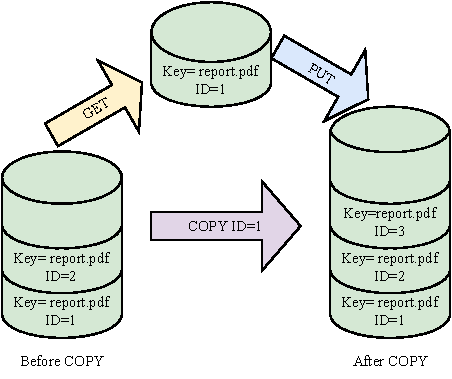
\includegraphics[scale=1.3]{../Figures/versioning_copy}
        \caption{COPY a previous version of an object}
        \label{fig:copy}
    \end{figure}
    A copy of a previous version can be made into the same \acrshort{s3} bucket by first using GET request to retrieve the required ID followed by a PUT request. A note-worthy point during this method is that, the old version isn't moved and made the current version, rather a new object with a new unique ID is PUT into the bucket that is a copy of the requested version.
    \begin{figure}[H]
        \centering
        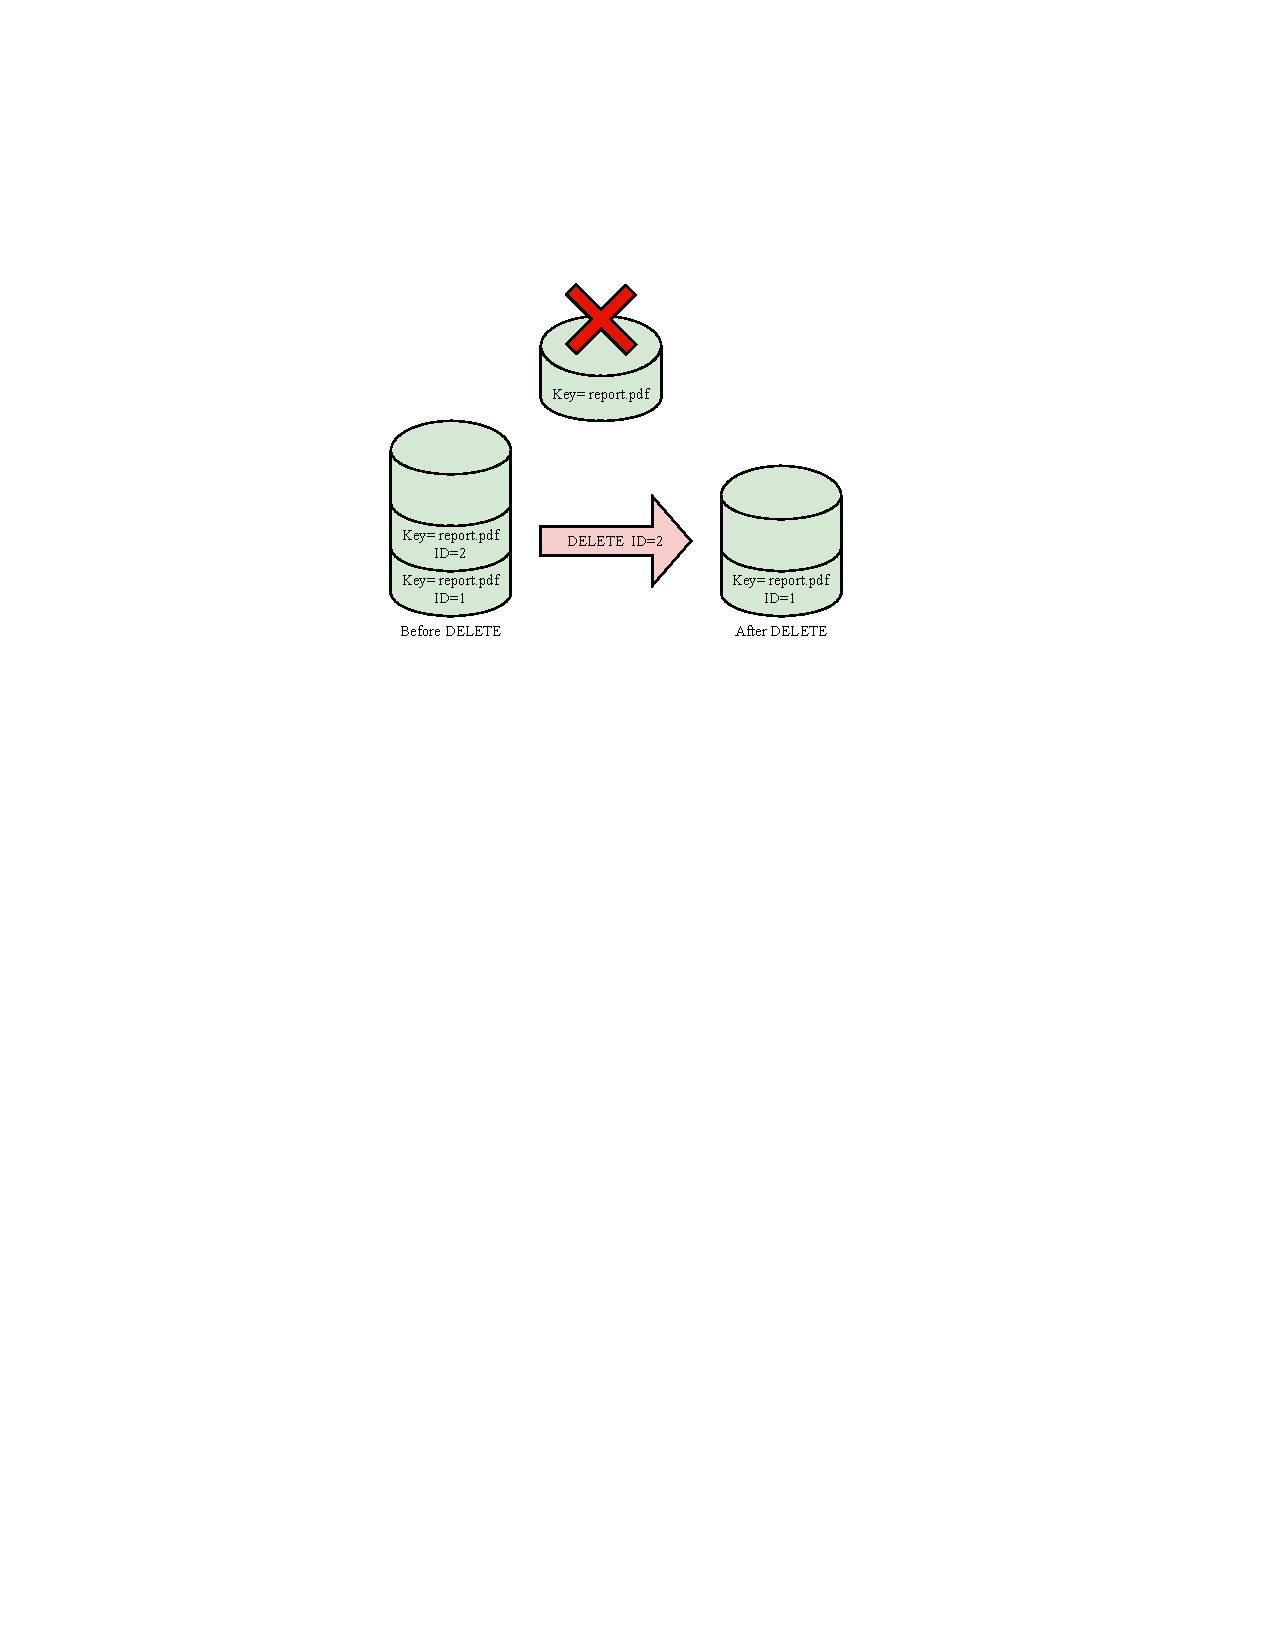
\includegraphics[scale=1.3]{../Figures/versioning_delete_permanent}
        \caption{Permanently DELETE the current version of an object}
        \label{fig:delete_permanent}
    \end{figure}
    Unlike Figure~\ref{fig:delete}, where a general DELETE request inserts a delete marker as the current version, if the user specify the ID of the version that they wish to delete, it is deleted permanently. This can be used to some extent restore the immediately previous version of the object, but if there are multiple versions existing, and the need is to restore a version that is quite old, multiple versions of the object would need to be deleted, which might not be what the user wants.

    \section{AWS Glacier}
    \acrshort{aws} Glacier is a low-cost, secure and durable storage class under \acrshort{aws} \acrshort{s3} storage classes, mostly used for data archiving purpose. As the name suggests, \acrshort{s3} Glacier is used to store cold data, a term commonly used for data that is archived or infrequently accessed but preserved for future access. Many organizations have the need of storing cold data but surely won't want high-cost storage services to do so. To keep the cost of \acrshort{aws} Glacier as low as possible, \acrshort{aws} provides data retrieval in one of three ways,
    \begin{enumerate}
        \item \textbf{Bulk retrieval:} To recover large among of data in 5 to 12 hours.
        \item \textbf{Standard retrieval:} To recover data in 3 to 5 hours.
        \item \textbf{Expedited retrieval:} To recover data within 5 minutes.
    \end{enumerate}
    Some use cases of \acrshort{aws} Glacier are,
    \begin{enumerate}
        \item \textbf{Digital preservation:} Many governmental firms and offices utilize Glacier service for digital preservation of the important data.
        \item \textbf{Regulatory and compliance archiving:} Since health and financial firms require large amount of regulatory and compliance archives, they use Glacier services.
        \item \textbf{Tape replacement:} With large upfront investment and maintenance needs, tape archiving can be replace by Glacier archiving.
        \item \textbf{Media assets storage:} Large media files that require a lot of space are stored in affordable Glacier buckets.
    \end{enumerate}
    Some of the benefits of \acrshort{aws} Glacier are,
    \begin{enumerate}
        \item \textbf{Durability and scalability:} Since \acrshort{aws} Glacier is distributed across at lease three availability zones, the durability of the storage is unquestioned. Similarly, organizations can scale their cloud archives as per their requirements.
        \item \textbf{Lower cost:} \acrshort{aws} Glacier is one of the lowest-cost storage classes and also employs pay-as-you go, hence reducing the cost tremendously.
        \item \textbf{Security:} Glacier has support of various compliance standards and encryption that allow secure storage at low cost.
        \item \textbf{Retrieval options:} As mentioned above, there are different options that a client can choose from while retrieving their data hence giving them choice based on retrieval time and cost.
    \end{enumerate}

    \section{Static Website Deployment on AWS S3}
    To deploy static websites on \acrshort{aws} \acrshort{s3}, users need to create a storage bucket where the static code (\acrshort{html}, \acrshort{css}, \acrshort{js}) files are kept as objects. Necessary policies are then created for the public access of these static files and a \acrshort{s3} url for the \acrshort{html} object makes the website accessible over the internet.\\
    For this report, a simple \acrshort{html} file is used.
    \lstinputlisting[language=HTML,style=customStyle, caption={HTML code for the static website}]{index.html}
    Hosting a static website isn't however limited to a single \acrshort{html} file, rather different styling codes in \acrshort{css} and functional codes in \acrshort{js} codes are necessary. It should be noted that the entire project must be made public so that the static website functions properly. Similarly, if there are any media assets that are used in the website, they too need to be accessible publicly. The steps to host a static website on \acrshort{aws} \acrshort{s3} include,
    \begin{enumerate}
        \item Create a bucket and make sure the bucket can have public objects.
        \item Upload code files to the bucket and make the files public.
        \item Access the website using the \acrshort{s3} object url.
    \end{enumerate}
    
    \step{1}{Log in to \acrshort{aws} console}
    Firstly, log in to the \acrshort{aws} console using a valid user with access to \acrshort{s3} services. In this report, the log in was done using the sandbox account from \acrshort{aws} Academy.\newpage
    \step{2}{Open \acrshort{s3} service from the \acrshort{aws} services list}
    Search for \acrshort{s3} service in the search box and select \acrshort{s3} service to proceed.\newpage
    \step{3}{Create a \acrshort{s3} bucket}
    To create a \acrshort{s3} bucket select any one of the \textit{Create bucket} buttons.
    \newpage
    \step{4}{Set an unique bucket name}
    Bucket names must be unique without using any spaces or uppercase letters. Choose an appropriate name that will be easy to remember. For this example, the name chosen is \textit{static-website-hosting-assignment}.
    \newpage
    \step{5}{Grant public access to bucket}
    Unselect the \textit{Block all public access} option. Also select the \textit{I acknowledge that the current settings might result in this bucket and the objects within becoming public} option.
    \newpage
    \step{6}{Complete bucket creation}
    Click on the \textit{Create bucket} button to complete the bucket creation process.
    \newpage
    \step{7}{Select the created bucket}
    Confirm that the bucket is created and then select the bucket to proceed.
    \newpage
    \step{8}{Upload objects to the bucket}
    Click on the \textit{Upload button} to start the upload process.
    \newpage
    \step{9}{Upload a file or a folder as needed}
    Click on the \textit{Add files} or \textit{Add folder} button as necessary. Since there is only one file for this example, \textit{Add files} is selected.
    \newpage
    \step{10}{Select the file to upload}
    Using the prompt that pops up, browser the local directory and select the required file to upload.\newpage
    \step{11}{Upload selected file}
    Click \textit{Upload} button to start uploading the selected file.\newpage
    \step{12}{Confirm the file upload}
    Confirm that the file upload succeeded and then click \textit{Close} button.
    \newpage
    \step{13}{Make the object public}
    Select the uploaded file, and click \textit{Actions} to open a drop-down menu. Scroll to the bottom of the menu and select \textit{Make public} option.
    \newpage
    \step{14}{Review the selected object}
    Review the selected object, and click \textit{Make public} button to proceed.
    \newpage
    \step{15}{Confirm public access}
    Confirm that the public access status is edited correctly and then click \textit{Close} button.
    \newpage
    \step{16}{Copy the object url}
    Select the object and click \textit{Copy URL} button.
    \newpage
    \step{17}{Visit the url and access the website}
    Paste the copied url in the browser search bar and go to the url. The static website is accessible using this url over the internet. 
    \end{document}